\chapter{Flow entry verification and Fake link detection}
This work focuses on the problem that a compromised switch will bring and presents the methods to detect such a switch. This work involves two parts: \textit{flow entry verification} and \textit{fake link detection}. We will define the threat model that both parts share, and explain them along with their attack scenarios and detection algorithms.

\section{Threat model and Attack scenario}
In this work, we assume the following scenario of compromising a switch in the threat model:
\begin{enumerate}
\item
One controller is used, and only one OpenFlow switch is compromised. No cooperation among multiple compromised switches for attacks will happen.
\item
The switches are able to access the Internet. 
\item
Other parts of the network such as the controller, other switches and hosts function normally. Any potential flaw is unintentional and is out of the scope of this work.
\item
An attacker cannot totally change the way of switch processing or core mechanism, but only perform the attack by modifying flow entries or forge LLDP to cause fake links.
\item
Initially, the network is all clean, and nothing is compromised. The attacks take place some time after the whole network is established.
\end{enumerate}

The attack scenarios beyond the assumptions such as multiple compromised switches, as well as possible circumvention, will be discussed in Section~\ref{Further_discussion}.

\section{Flow entry verification}
In the first part of this work, we propose a method to detect if the flow entries of a switch work as expected. The method is inspired by \cite{CKGL15}. The method in this work has two main enhancements. First, it reduces the number of detection packets required, and therefore increases the efficiency significantly. Second, the additional flow entries we need to install is less than the previous method, resulting in lower cost for setting up and cleaning up. 

\subsection{Detection method}
\label{Detection_method}
The main idea of the method is to assemble a packet that will go through a series of switches by matching the match fields in the flow entries of those switches. Then the packet will be sent into the network, go through a serie of flow entries inside switches, and should be sent back to the controller finally if nothing goes wrong. For this purpose, we take advantage of the network-wise visibility provided by the controller. 

The flow chart of the flow entry detection process in the controller is shown in Figure~\ref{flow_entry_detection_flowchart}. In the first step of this flowchart, we try to find ``aggregated groups''. An aggregated group is able to aggregate multiple match fields together. It consists of one flow entry of each switch in the same group. Assume there is a serie of switches, $S_{1..n}$ in a same aggregated group. Each switch will contain a flow entry selected according to our self-defined condition that has the output action forwarding to next switch. For example, starting from $S_{1}$, we try to find a flow entry that matches the requirement inside $S_{1}$, it has output action to $S_{2}$. We move on to $S_{2}$ and try to find an entry which also meets the requirement, it has forwarding action to $S_{3}$, and so on. Eventually, when a switch $S_{n}$ does not contain any flow entry that fits the requirement, a new flow entry with action forwarding to the controller will be installed on $S_{n}$.

The requirement condition that the flow entries in the same aggregated group must satisfy is called \textit{aggregation conditions}:

\begin{enumerate}
\item
Either one other flow entry that has exactly the same match field and same value, or there is no other flow entry with the same match field in different switches of the same group.
\item
There is no switch that has more than one entry selected in the same group, which might cause cycle.
\end{enumerate}

\begin{figure}[H]
\begin{center} 
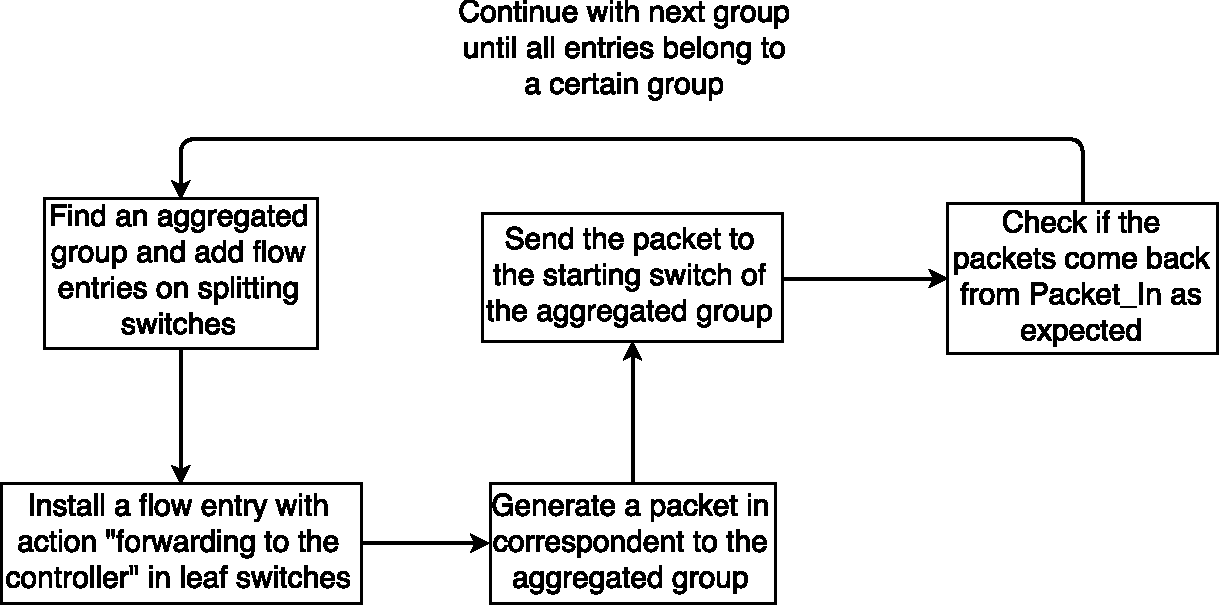
\includegraphics[width=1\textwidth]{figures/flow_entry_detection_flowchart.pdf}
\end{center}
\caption{The flow chart of the flow entry detection process.}
\label{flow_entry_detection_flowchart}
\end{figure} 

With the complete view of network provided by the controller and the aggregation condition, the controller is able to construct a detection packet to be sent from the first flow entry all the way down to the last flow entry during an aggregated group defining process. After sending it to the first switch of the aggregated group, it should come back to the controller, indicating that all the flow entries inside this aggregate group work as expected. 

Figure~\ref{aggregated_group} illustrates an aggregated group and the content of a constructed packet. The flow entries connected by arrows belong to the same group. After determining an aggregated group, the controller constructs a packet according to the match fields of flow entries inside the aggregated group. With the aggregation condition, it will match every flow entry inside the aggregated group. In the example figure, we have a controller, three switches, which are S1,S2 and S3, and a packet waiting to be constructed. In S1, there is a flow entry that contains match field eth\_dst, match value A and output action to S2. In S2, the flow entry has match field ipv4\_src, match value B and output action to S3. Initially in S3, there is no flow entry that matches the aggregation condition of this aggregated group, so we use it as the ending node and set a flow entry with arbitrary match field (in the example, arp\_op is used) and value C in order to notify the controller. According to these match fields, the constructed packet will contain eth\_dst as A, ipv4\_src as B and arp\_op as C. Then the packet is sent to S1, and will match to the flow entry and be sent to S2. After this, the packet will match the second flow entry in the aggregated group and be sent to S3. Finally, when it reaches the last flow entry made by us, it will be sent back to the controller, and the processing of this aggregated group is done.

\begin{figure}[H]
\begin{center}
\includegraphics[width=1\textwidth]{figures/aggregated_group.png}
\end{center}
\caption{An aggregated group and constructed packet.}
\label{aggregated_group}
\end{figure}

The process of generating a packet is done along with defining one aggregated group, the pseudo-code of it is as follow:

\begin {tcolorbox}[blanker,float=tbp,
grow to left by=1cm, grow to right by=1cm]
\begin{algorithm}[H]

  \caption{Packet generating process.}
  \begin{algorithmic}[1]
    \Require
      Information of all switches, $switches$;
      Global visited status of every flow entry, $visited\_entry$;
      Visited status of every switch in a aggregation group, $visited\_switch$
      An under-constructing packet that is initially empty, $packet$; 

    \Function{flow\_entry\_traversal}{switches}
      \ForAll{$switch$ in $switches$}
        \ForAll{$entry$ in $switch$}
          \State Extract $match\_field$, $match\_value$, $action$, $cookie$ from $entry$;
          \State $entry\_id \gets \textit{cookie}$; //use cookie as entry identifier
          \State 
          \State Extract $next\_switch$ from $action$;
          \If{NOT $visited\_entry$[$entry\_id$] and NOT $visited\_switch$[$next\_switch$]}
            %\State $\textit{visited\_switch}[\textit{switch}] \gets true$;
            \State $\textit{visited\_entry}[\textit{entry\_id}] \gets true$;
            \State $packet[\textit{match\_field}] \gets \textit{match\_value}$;
            \State $\textit{complete\_packet} \gets \Call{packet\_gen}{\textit{match\_field}, \textit{match\_value}, \textit{action}, \textit{packet}}$;
            \State Send $\textit{complete\_packet}$ with PACKET\_OUT;
          \EndIf
      \EndFor
        \EndFor
    \EndFunction
    \State
    \Function{packet\_gen}{match\_field$, match\_value$, action$, packet$}      
      \ForAll {$entry$ in $next\_switch$}
        \State Extract $match\_field$, $match\_value$, $action$, $cookie$ from $entry$;
        \State Extract $next\_switch$ from $action$; 
  \algstore{packet_generating}
  \end{algorithmic}
\end{algorithm}
\end{tcolorbox}

\begin {tcolorbox}[blanker,float=tbp,
grow to left by=1cm, grow to right by=1cm]
\begin{algorithm}[H]
  \begin{algorithmic}[1]
  \algrestore{packet_generating}
        \State $\textit{entry\_id} \gets \textit{cookie}$;
        \If{NOT $visited\_entry$[$entry\_id$] and NOT $visited\_switch$[$next\_switch$]}  
          \State $\textit{visited\_entry}[\textit{entry\_id}] \gets true$;
          \State $\textit{visited\_switch}[\textit{next\_switch}] \gets true$;
          \If{$packet$[$match\_field$] is set and $packet$[$match\_field$] = $match\_value$}            
            \State \Return \Call{packet\_gen}{$match\_field$, $match\_value$, $action$, $packet$};
          \ElsIf{$packet$[$match\_field$] is not set}
            \State $\textit{packet}[\textit{match\_field}] \gets \textit{match\_value}$;
            \State \Return \Call{packet\_gen}{$match\_field$, $match\_value$, $action$, $packet$};
          \EndIf
        \EndIf
      \EndFor
      \State Install new flow entry with action forwarding to controller into $next\_switch$;
      \State $\textit{visited\_switch} \gets EMPTY$;
      \State \Return $packet$;
    \EndFunction
  \end{algorithmic}
\end{algorithm}
\end{tcolorbox}

In order to optimize the number of necessary detection packets, the whole network should be covered with the minimum number of aggregated groups. By taking switches as vertex and forwarding actions as edges, it forms a complex graph problem. It is more complex than Longest path problem, which is also np-complete in time complexity. Inspired by Euler Path, we calculate the number that every vertex is destination of some edges, and use it as visiting priority as a approximation method. The reason behind the thought is that, the vertex who is treated as the destination the least time should be used as start point in order to reduce the number of necessary groups.

The cookie is used to identify every unique entry in different switches. When defining an aggregated group, we start with an unvisited flow entry that currently is treated as destination the least time, seek for an unvisited flow entry that matches the aggregation condition, and go to the next flow entry in other switch according to the output action recursively. Eventually, switch that does not have any entry that matches the aggregation condition for this group is reached, the aggregated group defining process ends, and a packet will be generated in correspondent to the flow entries inside the aggregated group. According to the aggregation condition, every aggregated group will be mutual exclusive. By going through through all the flow entries inside the switches, we should be able to cover all of the flow entries with multiple aggregated group. After all of the flow entries with output action is visited and belong to certain aggregated groups, and all the flow entries will be verified after sending the same number of packets with the number of aggregated groups. 

\subsection{Additional consideration of flow entry verification method}
\label{Further_discussion}

In real case, the variety of the conditions aggregation may be much more complicated. A flow entry might have multiple match fields. Multiple flow table may also cause similar problem. When the action in a flow entry send the packet to next table for further processing. The packet is also matched against more than one match field. These kind of situations can still be covered by our method with some modification. 
If all the fields and values match the under-constructing packet, we process it according to first aggregation rule. Otherwise we fill the packet with all of those match fields. If any match fields is already taken with different value, it will be ignored for this turn of aggregation process and fill the match fields in another packet that has no conflict field. However, the number of flow entries aggregated in a packet is reduced, and so is the effectiveness. Another condition is the conjunction action that ties groups of individual flows with same match field and different value into ``conjunctive flows'' and reduce the number of flow entry \cite{OVS_OFCTL}. It can also be dealt in a specific way. However, the main purpose of our method is to show the effectiveness of flow entry aggregation method. We will only demonstrate with the most simple condition, which is a match field that has one value.

It is certainly possible that more than one switch are made by the same manufacturer or have the same software version in the same network, so multiple switches share the same vulnerabilities and may be compromised simultaneously. However, cooperation between multiple compromised switches complicates the scenario significantly. Taking our own method as an example, suppose there are two compromised switches, CS1 and CS2, which are neighbors to each other, and both contain an entry in the same aggregation group. When CS1 receives the detection packet and forwards it to other place maliciously, it sends one copy of detection packet to CS2, the other copy back to the controller, and the rest of the detection process will continue without raising any suspicion\sout{\red{Since the controller does not receive the detection packet, is it possible to raise a suspicion here?}}. In order to simplify the case as a starting point for developing the detection method, we assume only one switch inside the network is compromised.

Suppose an attacker is able to add, remove, or modify the entries in the flow tables of a compromised
switch without notifying the controller, so packets may be forwarded to an undesired destination. The proposed method is intended to detect this behavior with high efficiency. In this method, only output action of packets is considered. Other actions such as dropping packets, setting field, changing TTL will be ignored \sout{\red{Cann't they (e.g., dropping packets) be detected?}}. Although there are reasonable methods to deal with these actions, for example, to detect packet dropping, we can add timeout checking function, such detection function is irrelevant to our main method and is not implemented in our work.

In this detection method, there is another important consideration: the controller must maintain unpolluted information of all flow entries. It is not reliable for a controller to obtain flow entry information by querying switches because a switch may be malicious and forge a fake response that gives false information about the flow entries. It is also possible to initiate OpenFlow message such as adding a new flow entry, resulting in adding a malicious entry without raising any alarm. However, it also means that it makes this malicious behavior known to controller and is quite noticeable.

\section{Fake link detection}

-----
When a switch is compromised, an attacker is surely able to drop LLDP and causes DOS. However, it is very noticeable. We will focus on the MITM types of attack
-----
\subsection{Attack scenario}
\subsection{Detection method}


-----------------------------------------------------------

Below is our attack scenario assumption: 
- The control channel is properly protected with TLS protocol, meaning
that it provides confidentiality for the control traffic as well as mutual
authentication between the controller and switches.

Packet pair

- The dispersion in normal vs attack scenario, regardless of congestion

----
If this is not the case, further narrow down process is needed to find the location of the compromised switch XXXXXXXXXXXXXXXXXXXXXXX.
----

Time and space complexity


Packet forwarded to non-existent ports are just dropped
